\section{Protocol and Architecture Effects}
\label{sec:protocol-results}

\subsection{RQ1: Does Graph Visibility Change the Leaderboard?}

On Elliptic, it changes the leading model in the evaluated three-model set. Under strict-inductive visibility, GraphSAGE has mean AUPRC $0.6114$, ahead of GCN ($0.4666$) and MLP ($0.4522$). Under isolated-inductive visibility, GCN leads at $0.5605$, followed by GraphSAGE at $0.4797$ and the unchanged MLP at $0.4522$. Thus the top-ranked model switches from GraphSAGE to GCN without changing temporal masks, training data, seed set, or selection metric.

DGraphFin does not show the same top-rank switch. GraphSAGE remains first, but its mean AUPRC falls from $0.0227$ to $0.0178$. MLP remains at $0.0140$, while GCN changes from $0.0116$ to $0.0118$. A protocol can therefore alter the margin or the winner; the Elliptic result is not evidence that every graph-fraud leaderboard must reverse.

\begin{table*}[t]
\caption{Paired AUPRC effects of strict versus isolated graph visibility over ten shared seeds. $\Delta$ is isolated minus strict; intervals are deterministic 95\% bootstrap intervals. Holm correction covers the six AUPRC comparisons.}
\label{tab:rb09-effects}
\centering
\footnotesize
\setlength{\tabcolsep}{3.2pt}
\begin{tabular}{@{}llrrrrrrr@{}}
\toprule
Dataset & Model & Strict & Isolated & $\Delta$ & 95\% CI & Rel. $\Delta$ (\%) & $d_z$ & Holm $p$ \\
\midrule
DGraphFin & GCN & 0.0116 & 0.0118 & +0.0002 & [-0.0013, +0.0019] & +1.6 & +0.07 & 1.000 \\
DGraphFin & MLP & 0.0140 & 0.0140 & +0.0000 & [+0.0000, +0.0000] & +0.0 & +0.00 & 1.000 \\
DGraphFin & GraphSAGE & 0.0227 & 0.0178 & -0.0049 & [-0.0064, -0.0033] & -21.5 & -1.88 & 0.016 \\
Elliptic & GCN & 0.4666 & 0.5605 & +0.0938 & [+0.0790, +0.1082] & +20.1 & +3.77 & 0.012 \\
Elliptic & MLP & 0.4522 & 0.4522 & +0.0000 & [+0.0000, +0.0000] & +0.0 & +0.00 & 1.000 \\
Elliptic & GraphSAGE & 0.6114 & 0.4797 & -0.1317 & [-0.1422, -0.1211] & -21.5 & -7.40 & 0.012 \\
\bottomrule
\end{tabular}
\end{table*}


\begin{figure*}[t]
  \centering
  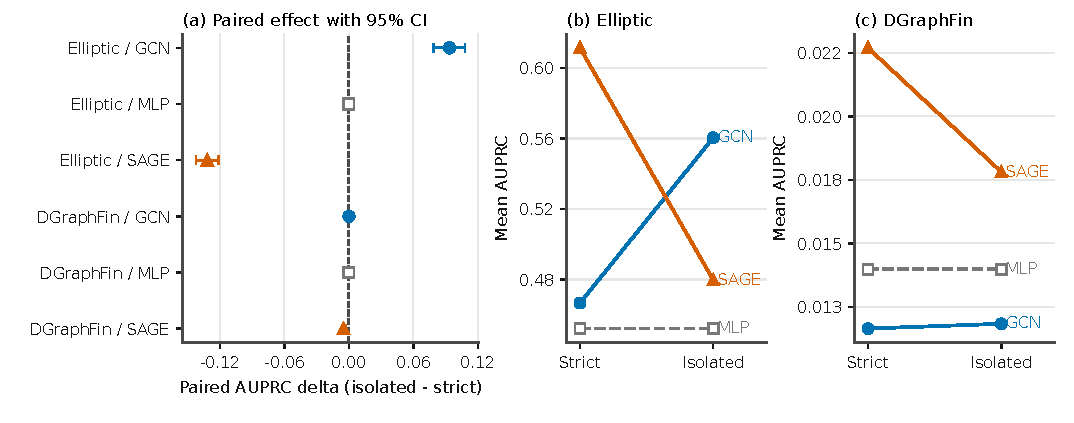
\includegraphics[width=\textwidth]{figures/fig02_protocol_architecture_effects.pdf}
  \caption{Strict-to-isolated AUPRC effects over ten paired seeds. Horizontal intervals are deterministic 95\% bootstrap intervals. The MLP control is unchanged; graph-model direction and magnitude depend on architecture and dataset.}
  \label{fig:protocol-effects}
\end{figure*}

\subsection{RQ2: Are Visibility Effects Architecture-Dependent?}

They are. GraphSAGE loses $21.5\%$ of strict AUPRC on both datasets. The paired absolute changes are $-0.1317$ on Elliptic (95\% CI $[-0.1422,-0.1211]$, $d_z=-7.40$, Holm $p=0.012$) and $-0.0049$ on DGraphFin (95\% CI $[-0.0064,-0.0033]$, $d_z=-1.88$, Holm $p=0.016$). The similar relative percentage masks a large difference in absolute task scale.

GCN moves in the opposite direction on Elliptic: $+0.0938$ AUPRC, or $+20.1\%$ (95\% CI $[0.0790,0.1082]$, $d_z=3.77$, Holm $p=0.012$). Its DGraphFin change is $+0.0002$ with an interval crossing zero and Holm $p=1$. MLP is numerically identical under the two graph views on both datasets, as expected from the intervention.

These patterns reject a uniform ``graph structure helps'' or ``graph structure hurts'' account. Isolating held-out nodes removes train-to-held-out message paths while keeping features, labels, and masks fixed. The result measures sensitivity to that visibility contract. It does not by itself identify homophily, oversmoothing, degree shift, or another mechanism as the cause. For model selection, the practical point is simpler: a validation winner obtained with one graph view is not automatically the winner for another deployment view.
